\begin{enumerate}[label=\arabic*.,ref=\theenumi]
\numberwithin{equation}{enumi}
\renewcommand{\thefigure}{\theenumi.\arabic{figure}}

\item For the circuit in Fig. \ref{fig:ee18btech11050_f1} (ignore the amplitude stabilization circuitry), find the loop gain GH by breaking the circuit at node X. 

\begin{figure}[!ht]
	\begin{center}
		\resizebox{\columnwidth}{!}{\begin{circuitikz}
\ctikzset{bipoles/length=1cm}

\draw 
(0, 0) node[op amp] (opamp) {}
(opamp.-) -- (-2.5,0.35) to[R,l_=$10k\ohm$,*-*] (-3.5, 0.35) to [C,l_=$16nF$,*-*] (-5,0.35) to [C,l_=$16nF$,*-*] (-6, 0.35) to [C,l_=$16nF$,*-*] (-7, 0.35) {}
(opamp.+) -- (-1.0,-0.35) node[ground]{}
(-4.8,0.35) -- (-4.8,-0.8) to [R,l_=$R$,*-*](-4.8,-1.8) --(-4.8,-2.3)node[ground] {}
(-6,0.35) -- (-6,-0.8) to [R,l_=$R$ ,*-*](-6,-1.8) --(-6,-2.3) node[ground] {}
(opamp.-) -- (-0.9,1.5) to [D, l_=$D_1$, *-*](1,1.5)to [R,l_=$R_2$, *-*](1,0.25)--(1,0){}
(1,0) to[R,l_=$R_3$, *-*](1,-2)to[D,l_=$D_2$,*-*](-1,-2)--(-2,-2) --(-2,0.35){}
(1,-2) to[R,l_=$R_4$, *-*](1,-4) node[vee]{$V^-$}
(1,1.5) to[R,l_=$R_1$, *-*](1,3) node[vcc]{$V^+$}
(opamp.out) to (2.5,0)--(2.5,7) -- (-7,7) -- (-7,0.35){}
(2.5,0)--(3,0){}
(2.5,0)--(2.5,5) to [potentiometer,n=mypot,l_=$P_1$](0.5,5) to  [R,l=$100k\ohm$](-0.6,5) --(-0.9,5)--(-0.9,1.5){}
(mypot.wiper) --(2,4.6)  --(2,5){}

(-0.3,5.5)coordinate(left)
(2,5.5)coordinate(right)
(-0.3,4.8)coordinate(bottoml)
(2,4.3)coordinate(bottomr)

node[fit=(left)(right)(bottoml)(bottomr),draw, dashed, label={$R_f$},inner sep=10pt] {}
node at(3.3,0){$V_0$}
node at(-7.5,0.1){$X$}
node at(-4.1,-1.5){$10k\ohm$}
node at(-6.6,-1.8){$10k\ohm$}
node at(-3,-0.1){$R$}
node at(-4.2,-0.2){$C$}
node at(-5.5,-0.2){$C$}
node at(-6.5,-0.2){$C$}
;\end{circuitikz}
}
	\end{center}
\caption{}
\label{fig:ee18btech11050_f1}
\end{figure}

\item \solution
The equivalent control system representation of Oscillator circuit is shown in Fig. \ref{fig:ee18btech11050_f4}. Oscillator circuits do not have input.
\begin{figure}[!ht]
	\begin{center}
		\resizebox{\columnwidth}{!}{\tikzstyle{block} = [draw, rectangle, 
    minimum height=3em, minimum width=6em]
\tikzstyle{sum} = [draw, circle, node distance=1cm]
\tikzstyle{input} = [coordinate]
\tikzstyle{output} = [coordinate]
\tikzstyle{pinstyle} = [pin edge={to-,thin,black}]

\begin{tikzpicture}[auto, node distance=2cm,>=latex']
    \node [input, name=input] {};
    \node [sum, right of=input] (sum) {};
    \node [block, right of=sum] (controller) {$G$};
    \node [output, right of=controller] (output) {};
    \node [block, below of=controller] (feedback) {$H$};
    \draw [draw,->] (input) -- node {} (sum);
    \draw [->] (sum) -- node {$V_i$} (controller);
    \draw [->] (controller) -- node [name=y] {$V_o$}(output);
    \draw [->] (y) |- (feedback);
    \draw [->] (feedback) -| node[pos=0.99]{$+$}  node [near end] {$V_f$} (sum);
\end{tikzpicture}
}
	\end{center}
\caption{}
\label{fig:ee18btech11050_f4}
\end{figure}
After removing the amplitude stabilization circuitry, when we break the loop at X, from Fig. \ref{fig:ee18btech11050_f2} the value of gain
\begin{align}
    GH = \frac{v_o(j\omega)}{v_x(j\omega)}
\end{align}

\begin{figure}[!ht]
	\begin{center}
		\resizebox{\columnwidth}{!}{\begin{circuitikz}
\ctikzset{bipoles/length=1cm}

\draw 
(0, 0) node[op amp] (opamp) {}
(opamp.-) -- (-1.5,0.35) to[R,l_=$R$,*-*] (-2.5, 0.35) to [C,l_=$C$,*-*, i<=$i_x$] (-4,0.35) to [C,l_=$C$,*-*] (-5.5, 0.35) to [C,l_=$C$,*-*] (-7, 0.35) {}
(opamp.+) -- (-1.0,-0.35) node[ground]{}
(-5.5,0.35) -- (-5.5,-0.8) to [R,l_=$R$,*-*](-5.5,-1.8) --(-5.5,-2.3)node[ground] {}
(-4,0.35) -- (-4,-0.8) to [R,l_=$R$ ,*-*](-4,-1.8) --(-4,-2.3) node[ground] {}
(opamp.out) -- (2,0){}
(2,0)--(3,0){}
(2.5,0)--(2.5,2) to[R, l_=$R_f$, i<=$i_x$](-1,2) --(-1,2)--(-1,0.35){}

node at(3.3,0){$v_o$}
node at(-7,0.1){$v_x$}
node at(0.1,1.5){$+$}
node at(1.2,1.5){$-$}
node at(-1,0.1){$v_1$}

;\end{circuitikz}
}
	\end{center}
\caption{}
\label{fig:ee18btech11050_f2}
\end{figure}
\begin{align}
    v_1 = 0
\end{align}
\begin{align}
    \implies v_o = -i_xR_f
    \label{ee18btech11050_eq1}
\end{align}
\begin{align}
    v_a = \brak{\frac{1+sRC}{sC}}i_x
\end{align}
\begin{align}
    \implies v_b = \brak{R + \frac{3}{sC} + \frac{1}{s^2C^2R}}i_x
\end{align}
\begin{align}
    \implies v_x = \brak{R + \frac{6}{sC} + \frac{5}{s^2C^2R} + \frac{1}{s^3C^3R^2}}i_x
\end{align}

\begin{align}
    \implies\frac{v_x}{i_x} = \brak{R+\frac{6}{sC}+\frac{5}{s^2C^2R}+\frac{1}{s^3C^3R^2}}
\end{align}
From \eqref{ee18btech11050_eq1}
\begin{align}
    \frac{v_x}{v_o} = -\frac{R}{R_f}\brak{1+\frac{6}{sCR}+\frac{5}{s^2C^2R^2}+\frac{1}{s^3C^3R^3}}
\end{align}

\begin{align}
    \implies \frac{v_o}{v_x} = -\frac{R_fs^3C^3R^3}{R\brak{s^3C^3R^3+6s^2C^2R^2+5sCR+1}}
\end{align}
Substituting $s=j\omega$ gives us the transfer function
\begin{align}
    \frac{v_o}{v_x} = GH = \frac{\omega^2C^2R_fR}{(5-\omega^2C^2R^2)+j(6\omega CR-\frac{1}{\omega CR})}
    \label{ee18btech11050_eq2}
\end{align}

\item Find frequency of oscillation $f_0$.
\item \solution 
For system to oscillate at a frequency $\omega_0$, 
\begin{align}
    L(j\omega_0) = G(j\omega_0)H(j\omega_0) = 1
    \label{ee18btech11050_eq4}
\end{align}
\begin{align}
    \implies \angle(G(j\omega_0)H(j\omega_0)) = 0
\end{align}
\begin{align}
    \implies 6\omega_0 CR = \frac{1}{\omega_0 CR}
\end{align}
\begin{align}
    \implies \omega_0 = \frac{1}{\sqrt{6}CR}
\end{align}
\begin{align}
    \implies \omega_0 = 2551.55 rad/sec
\end{align}
\begin{align}
    \implies f_0 = 406.1 Hz
\end{align}
\item Find $R_f$ for oscillation to begin.
\item \solution From \eqref{ee18btech11050_eq4}
\begin{align}
    Re(G(j\omega_0)H(j\omega_0)) = 1
\end{align}
\begin{align}
    \implies \frac{R_f\omega_0^2C^2R}{5-\omega_0^2C^2R^2} = 1
\end{align}
\begin{align}
    \implies R_f = 29R
\end{align}
\begin{align}
    \implies R_f = 290 k\ohm
\end{align}
Thus, for the oscillations to begin,
\begin{align}
    R_f \geq 290 k\ohm
\end{align}
\item Tabulate your results.
\item \solution See table \ref{parameters}
\begin{table}[!ht]
\centering
%%%%%%%%%%%%%%%%%%%%%%%%%%%%%%%%%%%%%%%%%%%%%%%%%%%%%%%%%%%%%%%%%%%%%%
%%                                                                  %%
%%  This is the header of a LaTeX2e file exported from Gnumeric.    %%
%%                                                                  %%
%%  This file can be compiled as it stands or included in another   %%
%%  LaTeX document. The table is based on the longtable package so  %%
%%  the longtable options (headers, footers...) can be set in the   %%
%%  preamble section below (see PRAMBLE).                           %%
%%                                                                  %%
%%  To include the file in another, the following two lines must be %%
%%  in the including file:                                          %%
%%        \def\inputGnumericTable{}                                 %%
%%  at the beginning of the file and:                               %%
%%        \input{name-of-this-file.tex}                             %%
%%  where the table is to be placed. Note also that the including   %%
%%  file must use the following packages for the table to be        %%
%%  rendered correctly:                                             %%
%%    \usepackage[latin1]{inputenc}                                 %%
%%    \usepackage{color}                                            %%
%%    \usepackage{array}                                            %%
%%    \usepackage{longtable}                                        %%
%%    \usepackage{calc}                                             %%
%%    \usepackage{multirow}                                         %%
%%    \usepackage{hhline}                                           %%
%%    \usepackage{ifthen}                                           %%
%%  optionally (for landscape tables embedded in another document): %%
%%    \usepackage{lscape}                                           %%
%%                                                                  %%
%%%%%%%%%%%%%%%%%%%%%%%%%%%%%%%%%%%%%%%%%%%%%%%%%%%%%%%%%%%%%%%%%%%%%%

 

%%  This section checks if we are begin input into another file or  %%
%%  the file will be compiled alone. First use a macro taken from   %%
%%  the TeXbook ex 7.7 (suggestion of Han-Wen Nienhuys).            %%
\def\ifundefined#1{\expandafter\ifx\csname#1\endcsname\relax}


%%  Check for the \def token for inputed files. If it is not        %%
%%  defined, the file will be processed as a standalone and the     %%
%%  preamble will be used.                                          %%
\ifundefined{inputGnumericTable}

%%  We must be able to close or not the document at the end.        %%
	\def\gnumericTableEnd{\end{document}}


%%%%%%%%%%%%%%%%%%%%%%%%%%%%%%%%%%%%%%%%%%%%%%%%%%%%%%%%%%%%%%%%%%%%%%
%%                                                                  %%
%%  This is the PREAMBLE. Change these values to get the right      %%
%%  paper size and other niceties.                                  %%
%%                                                                  %%
%%%%%%%%%%%%%%%%%%%%%%%%%%%%%%%%%%%%%%%%%%%%%%%%%%%%%%%%%%%%%%%%%%%%%%

	\documentclass[12pt%
			  %,landscape%
                    ]{report}
       \usepackage[latin1]{inputenc}
       \usepackage{fullpage}
       \usepackage{color}
       \usepackage{array}
       \usepackage{longtable}
       \usepackage{calc}
       \usepackage{multirow}
       \usepackage{hhline}
       \usepackage{ifthen}

	


%%  End of the preamble for the standalone. The next section is for %%
%%  documents which are included into other LaTeX2e files.          %%
\else

%%  We are not a stand alone document. For a regular table, we will %%
%%  have no preamble and only define the closing to mean nothing.   %%
    \def\gnumericTableEnd{}

%%  If we want landscape mode in an embedded document, comment out  %%
%%  the line above and uncomment the two below. The table will      %%
%%  begin on a new page and run in landscape mode.                  %%
%       \def\gnumericTableEnd{\end{landscape}}
%       \begin{landscape}


%%  End of the else clause for this file being \input.              %%
\fi

%%%%%%%%%%%%%%%%%%%%%%%%%%%%%%%%%%%%%%%%%%%%%%%%%%%%%%%%%%%%%%%%%%%%%%
%%                                                                  %%
%%  The rest is the gnumeric table, except for the closing          %%
%%  statement. Changes below will alter the table's appearance.     %%
%%                                                                  %%
%%%%%%%%%%%%%%%%%%%%%%%%%%%%%%%%%%%%%%%%%%%%%%%%%%%%%%%%%%%%%%%%%%%%%%

\providecommand{\gnumericmathit}[1]{#1} 
%%  Uncomment the next line if you would like your numbers to be in %%
%%  italics if they are italizised in the gnumeric table.           %%
%\renewcommand{\gnumericmathit}[1]{\mathit{#1}}
\providecommand{\gnumericPB}[1]%
{\let\gnumericTemp=\\#1\let\\=\gnumericTemp\hspace{0pt}}
 \ifundefined{gnumericTableWidthDefined}
        \newlength{\gnumericTableWidth}
        \newlength{\gnumericTableWidthComplete}
        \newlength{\gnumericMultiRowLength}
        \global\def\gnumericTableWidthDefined{}
 \fi
%% The following setting protects this code from babel shorthands.  %%
 \ifthenelse{\isundefined{\languageshorthands}}{}{\languageshorthands{english}}
%%  The default table format retains the relative column widths of  %%
%%  gnumeric. They can easily be changed to c, r or l. In that case %%
%%  you may want to comment out the next line and uncomment the one %%
%%  thereafter                                                      %%
\providecommand\gnumbox{\makebox[0pt]}
%%\providecommand\gnumbox[1][]{\makebox}

%% to adjust positions in multirow situations                       %%
\setlength{\bigstrutjot}{\jot}
\setlength{\extrarowheight}{\doublerulesep}

%%  The \setlongtables command keeps column widths the same across  %%
%%  pages. Simply comment out next line for varying column widths.  %%
\setlongtables

\setlength\gnumericTableWidth{%
	83pt+%
	91pt+%
0pt}
\def\gumericNumCols{2}
\setlength\gnumericTableWidthComplete{\gnumericTableWidth+%
         \tabcolsep*\gumericNumCols*2+\arrayrulewidth*\gumericNumCols}
\ifthenelse{\lengthtest{\gnumericTableWidthComplete > \linewidth}}%
         {\def\gnumericScale{\ratio{\linewidth-%
                        \tabcolsep*\gumericNumCols*2-%
                        \arrayrulewidth*\gumericNumCols}%
{\gnumericTableWidth}}}%
{\def\gnumericScale{1}}

%%%%%%%%%%%%%%%%%%%%%%%%%%%%%%%%%%%%%%%%%%%%%%%%%%%%%%%%%%%%%%%%%%%%%%
%%                                                                  %%
%% The following are the widths of the various columns. We are      %%
%% defining them here because then they are easier to change.       %%
%% Depending on the cell formats we may use them more than once.    %%
%%                                                                  %%
%%%%%%%%%%%%%%%%%%%%%%%%%%%%%%%%%%%%%%%%%%%%%%%%%%%%%%%%%%%%%%%%%%%%%%

\ifthenelse{\isundefined{\gnumericColA}}{\newlength{\gnumericColA}}{}\settowidth{\gnumericColA}{\begin{tabular}{@{}p{83pt*\gnumericScale}@{}}x\end{tabular}}
\ifthenelse{\isundefined{\gnumericColB}}{\newlength{\gnumericColB}}{}\settowidth{\gnumericColB}{\begin{tabular}{@{}p{91pt*\gnumericScale}@{}}x\end{tabular}}

\begin{tabular}[c]{%
	b{\gnumericColA}%
	b{\gnumericColB}%
	}

%%%%%%%%%%%%%%%%%%%%%%%%%%%%%%%%%%%%%%%%%%%%%%%%%%%%%%%%%%%%%%%%%%%%%%
%%  The longtable options. (Caption, headers... see Goosens, p.124) %%
%	\caption{The Table Caption.}             \\	%
% \hline	% Across the top of the table.
%%  The rest of these options are table rows which are placed on    %%
%%  the first, last or every page. Use \multicolumn if you want.    %%

%%  Header for the first page.                                      %%
%	\multicolumn{2}{c}{The First Header} \\ \hline 
%	\multicolumn{1}{c}{colTag}	%Column 1
%	&\multicolumn{1}{c}{colTag}	\\ \hline %Last column
%	\endfirsthead

%%  The running header definition.                                  %%
%	\hline
%	\multicolumn{2}{l}{\ldots\small\slshape continued} \\ \hline
%	\multicolumn{1}{c}{colTag}	%Column 1
%	&\multicolumn{1}{c}{colTag}	\\ \hline %Last column
%	\endhead

%%  The running footer definition.                                  %%
%	\hline
%	\multicolumn{2}{r}{\small\slshape continued\ldots} \\
%	\endfoot

%%  The ending footer definition.                                   %%
%	\multicolumn{2}{c}{That's all folks} \\ \hline 
%	\endlastfoot
%%%%%%%%%%%%%%%%%%%%%%%%%%%%%%%%%%%%%%%%%%%%%%%%%%%%%%%%%%%%%%%%%%%%%%

\hhline{|-|-}
	 \multicolumn{1}{|p{\gnumericColA}|}%
	{\gnumericPB{\raggedright}\gnumbox[l]{\textbf{Parameter}}}
	&\multicolumn{1}{p{\gnumericColA}|}%
	{\gnumericPB{\raggedright}\gnumbox[l]{\textbf{Value}}}
\\
\hhline{|-|-}
	 \multicolumn{1}{|p{\gnumericColA}|}%
	{\gnumericPB{\raggedright}\gnumbox[l]{$\omega_0$}}
	&\multicolumn{1}{p{\gnumericColA}|}%
	{\gnumericPB{\raggedright}\gnumbox[l]{2551.55 rad/s}}
\\
\hhline{|-|-}
	 \multicolumn{1}{|p{\gnumericColA}|}%
	{\gnumericPB{\raggedright}\gnumbox[l]{$f_0$}}
	&\multicolumn{1}{p{\gnumericColA}|}%
	{\gnumericPB{\raggedright}\gnumbox[l]{406.1 Hz}}
\\
\hhline{|-|-}
	 \multicolumn{1}{|p{\gnumericColA}|}%
	{\gnumericPB{\raggedright}\gnumbox[l]{$R_f$}}
	&\multicolumn{1}{p{\gnumericColA}|}%
	{\gnumericPB{\raggedright}\gnumbox[l]{$290k\ohm$}}

\\



\hhline{|-|-|}
\end{tabular}

\ifthenelse{\isundefined{\languageshorthands}}{}{\languageshorthands{\languagename}}
\gnumericTableEnd

\caption{calculated parameters}
\label{parameters}
\end{table}

\item Verify results using Spice Simulation.

\item \solution Following readme provides instructions for simulation in spice

\begin{lstlisting}
codes/ee18btech11050/spice/README.md
\end{lstlisting}

The following netlist simulates the given circuit in \ref{fig:ee18btech11050_f1}

\begin{lstlisting}
codes/ee18btech11050/spice/ee18btech11050_sim.net
\end{lstlisting}

The following code plots the oscillator output from spice simulation, which is shown in fig \ref{fig:ee18btech11050_f6}

\begin{lstlisting}
codes/ee18btech11050/spice/ee18btech11050_sim.py
\end{lstlisting}

\begin{figure}[!ht]
\centering
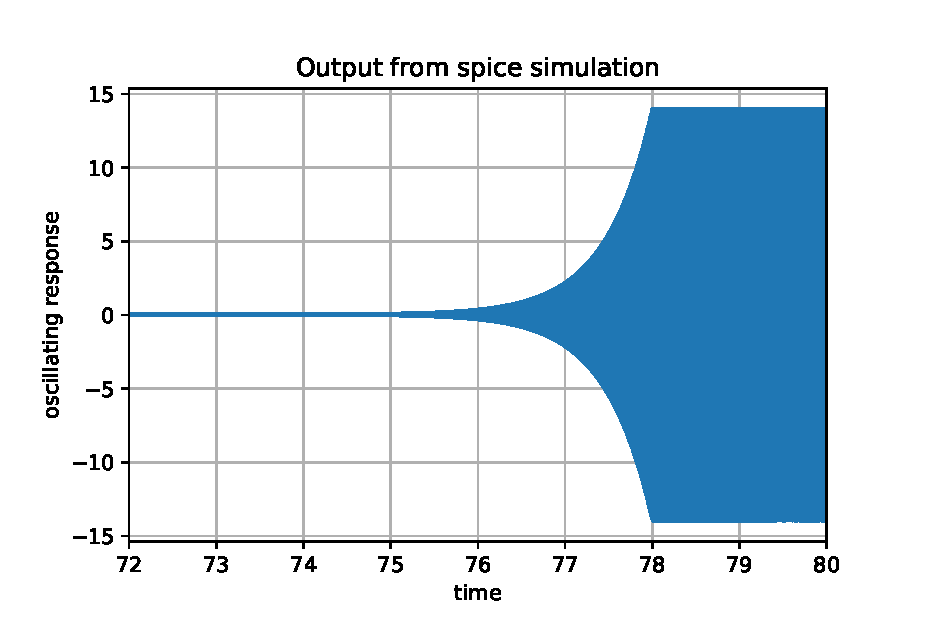
\includegraphics[width=\columnwidth]{./figs/ee18btech11050/ee18btech11050_sim.eps}
\caption{}
\label{fig:ee18btech11050_f6}
\end{figure}

The following code plots a part of spice output generated above, where a sinusoidal output can be clearly observed shown in fig \ref{fig:ee18btech11050_f7}

\begin{lstlisting}
codes/ee18btech11050/spice/ee18btech11050_sim2.py
\end{lstlisting}

\begin{figure}[!ht]
\centering
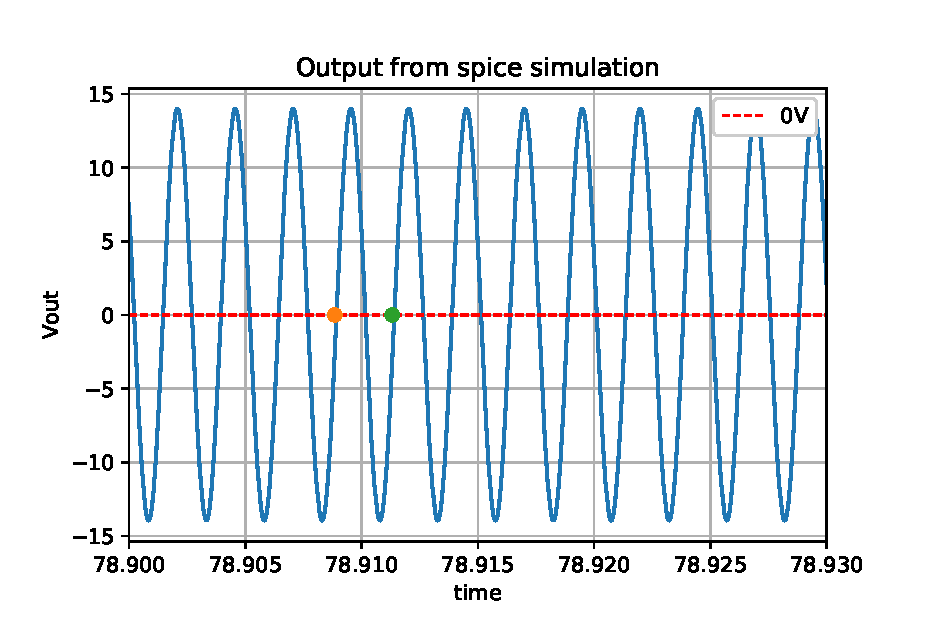
\includegraphics[width=\columnwidth]{./figs/ee18btech11050/ee18btech11050_sim2.eps}
\caption{}
\label{fig:ee18btech11050_f7}
\end{figure}

From fig \ref{fig:ee18btech11050_f7}, time period is calculated from one cycle:
\begin{align}
    T = 78.91131 - 78.908846 = 0.002464 sec
\end{align}
\begin{align}
    \implies f = 405.844 Hz
\end{align}

Hence frequency is verified through spice simulation.

\end{enumerate}
